\chapter{复合物筛选模型设计}
\label{chapter:gcnfilter}

\section{相关算法介绍}
\label{section:arithmetic}
\subsection{网络嵌入}
\label{subsection:nodeEmbedding}
\subsection{图卷积神经网络}
\label{subsection:GCN}
\subsection{图自编码器}
\label{subsection:GAE}
\section{算法总体流程}
\label{section:progress}

复合物筛选模型框架设计如图\ref{fig:main-process}所示;

\begin{figure}[htbp]
    \centering
    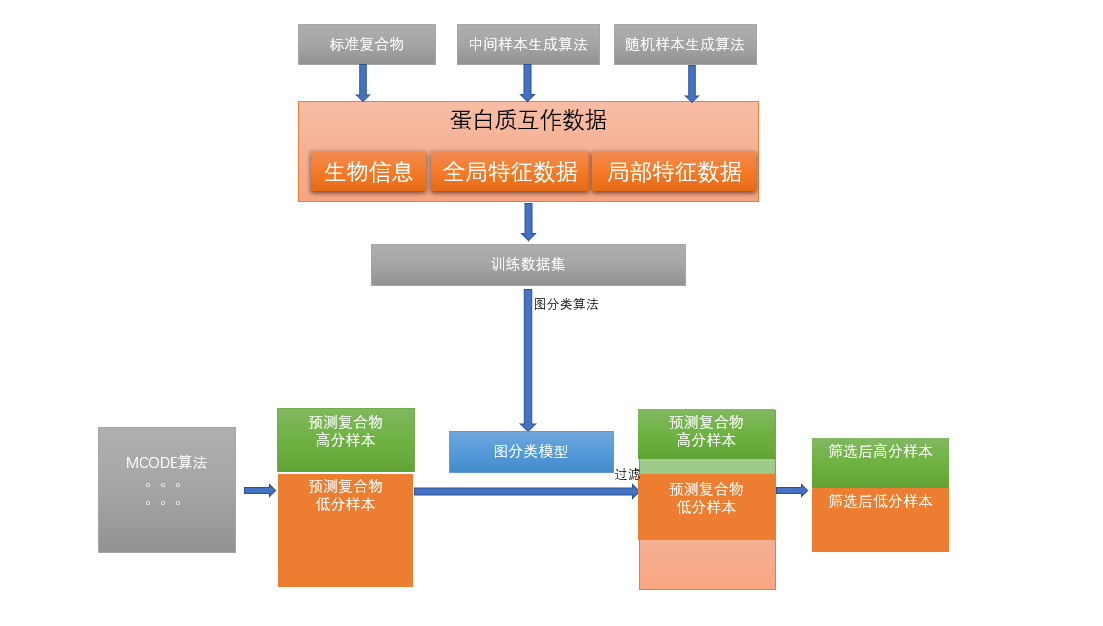
\includegraphics[width=14cm]{main-process}
    \caption{复合物筛选框架主体流程图}
    \label{fig:main-process}
\end{figure}

首先依照\label{section:datasetExtract}提出的数据集构建方法,对每一个复合物网络可以得到一个由复合物子图构成的数据集。该数据集中每一个复合物子图有和标准复合物的邻居相似性评分,总体分为四类复合物,分别为标准复合物、高评分预测复合物、低评分预测复合物和随机复合物。

第一阶段,提出合适的复合物筛选模型,并基于该数据集训练复合物分类模型\ref{section:GlobalfeatBaseModel}。

第二阶段,在蛋白质相互作用网络中得到复合物预测算法,如MCODE算法、clique算法等的预测结果。依据复合物分类结果的评价方法,在这些预测结果中,有一部分高分样本复合物预测符合预期结果,如图中绿色部分所示,其余部分为低分复合物样本,如图中红色部分所示。下一步利用复合物分类模型对所有的样本进行筛选,通过筛选的复合物符合模型学习到的复合物一般分布规律,筛选之后保留的复合物如图最终输出结果所示。

第三阶段,本文使用多种的复合物预测评价指标对筛选前后的总体样本进行综合评价。


\section{基于全局特征的模型}
\label{section:GlobalfeatBaseModel}
已有的基于监督学习的复合物预测算法,基本都是基于挖掘复合物子图的拓扑特征,比如图的密度、图的结点个数、平均度数等等,将图的所有拓扑特征置于一个向量中,构成一个$1\times N$的向量,用该向量代替子图,最后将向量用于训练分类模型。具体过程如图\ref{fig:entropy-classification}所示。

\begin{figure}[htbp]
    \centering
    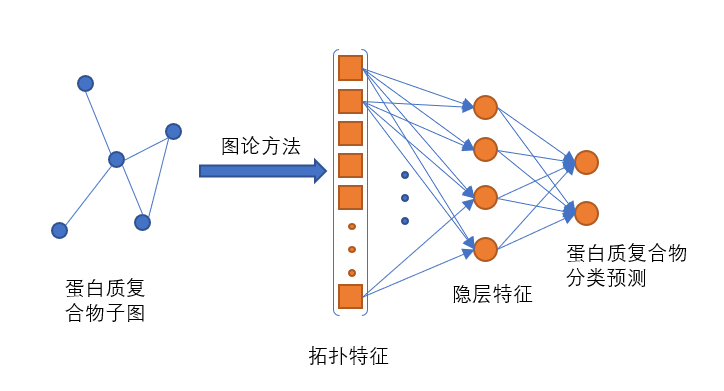
\includegraphics[width=14cm]{entropy-classification}
    \caption{基于图拓扑特征的蛋白质复合物分类模型}
    \label{fig:entropy-classification}
\end{figure}


但是蛋白质复合物中,有大部分是小复合物,其蛋白质个数小于5个。此类复合物的拓扑结构结构简单,提取的拓扑特征具有趋同性。随机的子图在结点数较少的情况下可能形成相同的拓扑特征,此时分类模型无法区分子图是否为真正的复合物。

为了解决该问题,在不引入额外的生物学信息的情况下,本文提出了基于全局特征的复合物分类模型。
蛋白质复合物网络是一个高维结构,可以通过挖掘蛋白质在网络中所处的位置和其周围相互作用关系挖掘蛋白质的潜在特征表示,将网络的高维数据转换为蛋白质的低维嵌入表示,成为每一个蛋白质初始的特征向量。

加入蛋白质嵌入特征之后,蛋白质复合物子图具有初始的结点特征向量。图卷积神经网络\label{subsection:GCN}具有动态融合结点特征的能力,已经广泛应用于图任务中。基于全局特征的模型加上了两层GCN网络对蛋白质结点特征进行融合,以蛋白质结点特征的平均池化作为蛋白质复合物特征的输出。

最终


现有的复合物预测模型


没有全局特征有什么局限性,为什么需要加入全局特征
怎么加入全局特征
GAE怎么做的,deepwalk怎么做的,node2vec怎么做的
深度自编码器为什么可以具有全局特征
全局特征具有之后,图卷积怎么进行的

对于复杂的拓扑结构,也能挖掘复杂特征。。。


\section{基于生物特征的模型}
\label{section:biofeatBaseModel}
生物特征为什么重要
生物特征加在哪里
图卷积通常是怎么做的,边的特征需要转换为点的特征
之后怎么操作

生物特征怎么处理,异常数据处理,过大数据归一化

\section{特征融合模型}
\label{section:fusionfeatBaseModel}
分析GCN的过程,发现这是一种融合的过程
以此提出融合点边的融合模型
考虑少量蛋白质特征,考虑图拓扑特征,图拓扑特征的计算参考\cite{yu_predicting_2014}
